%!TEX program = xelatex

\documentclass[a4paper,11pt]{article}

% Paquetes necesarios
%\usepackage[utf8]{inputenc}
\usepackage[spanish]{babel}
\usepackage{amsmath, amssymb}
\usepackage{graphicx} % Paquete para manejar imágenes
\usepackage{fancyhdr}
\usepackage{hyperref}
\usepackage{lipsum}
\usepackage{tocbibind}
\usepackage{geometry}
\geometry{left=3cm,right=2.5cm,top=2cm,bottom=2cm}
\usepackage{float}
\usepackage{fontspec}
\usepackage{caption}
\setmainfont{Times New Roman}

% Configuración del pie de página
\pagestyle{fancy}
\fancyhf{}
\fancyfoot[C]{\thepage}

\begin{document}
% portada
\begin{titlepage}
    \begin{center}
        \vspace*{1cm} 
        
\includegraphics[width=1\textwidth]{./uc3m.jpg}
        
        \vspace*{3cm} 
        
        {\LARGE Criptografía y seguridad informática\\[0.5cm]} 
        {\LARGE G24 - Entregable 1 \\[0.5cm]}
        
        \vspace*{6cm}
        
        \textbf{Javier Martín Pizarro: 100495861@alumnos.uc3m.es} \\[0.5cm]
        \textbf{Alberto Pascau Sáez: 100495775@alumnos.uc3m.es} \\[0.5cm]
        \textbf{Raúl Armas Seriña: 100495746@alumnos.uc3m.es} \\[0.5cm]
        
        \vspace*{3cm}
        \textbf{GitHub:
        \href{https://github.com/Albrtito/CriptCript.git}{Albrtito/CriptCript.git}}\\[0.5cm]

    \end{center}
\end{titlepage}

% Eliminamos el índice de contenidos
\tableofcontents
\vspace{2cm}
%\newpage


% Introducción sin numeración de capítulo
\section{Propósito de la aplicación. Estructura interna}

\subsection{Propósito de la aplicación}

La aplicación simula una página web, levantada en local por el propio usuario,
en la que se pueden crear desafíos criptográficos(\textit{challenges}) con algoritmos de cifrado
clásico.\\\\
A la hora de crear un desafío cada usuario podrá elegir el algoritmo con el que
cifrar su desafío.El objetivo de otros usuarios será resolver que algoritmo de
cifrado se ha utilizado y el valor de la clave del cifrado; para ayudar en el
descifrado de desafíos la applicación implementará herramientas de
criptoanálisis simples.\\
Cada desafío sera público o privado, dependiendo de la elección que haga su
autor en su creación.
\begin{itemize}
    \item \textbf{Desafío público:} cualquier usuario registrado tiene acceso a ellos.
    \item \textbf{Desafío privado:} solamente pueden ser compartidos con un
        único usuario. El creador del desafío selecciona qué usuario será capaz de verlo.
\end{itemize}

El propósito de esta aplicación es generar un sistema informático que cumpla
unos requisitos mínimos. Nótese que a medida que la práctica avance, esta lista
podrá verse modificada. Los requisitos para esta primera entregá incluyen las
necesidades mínimas de la práctica.
son:\begin{enumerate}
    \item El sistema debe de ser capaz de registrar y autenticar usuarios.
        Guardando su información confidencial correctamente cifrada(contraseñas).$\rightarrow$\textbf{Requisito de confidencialidad}
    \item El sistema debe ser capaz de permitir un inicio de sesión donde se sea capaz de obtener y comparar 
        los datos cifrados de los usuarios de la base de datos con los proporcionados por el cliente.
    \item El sistema debe de ser capaz de guardar y recuperar desafíos usando
        cifrado simétrico/asimétrico. 
        $\rightarrow$ \textbf{Requisito de confidencialidad}
    \item El sistema debe de ser capaz de permitir a un usuario $A$ leer el desafío creado por el usuario $B$ si este se lo ha compartido.
    \item El sistema debe de autenticar que los mensajes mandados por usuarios a la
        base de datos no han sido alterados y son de quien dicen ser $\rightarrow$ \textbf{Requisito de Integridad y
        Autenticidad}
    \item Para cumplir con el requisito 5 el sistema ha de implementar alguna
        forma de MAC o cifrado autenticado
    \item El sistema debe de ser capaz de mostrar en pantalla todos los
        desafíos, privados y públicos, específicos para cada usuario.
\end{enumerate}

\subsection{Estructura interna}

Esta aplicación consta de tres partes fundamentales:
\begin{itemize}
    \item \textbf{Frontend:} esencial para la experiencia de usuario. Actua como interfaz entre el cliente y el backend.
    \item \textbf{Backend:} donde se encuentra la API, implementada usando
        Flask. Todos los mecanismos de cifrado, autenticación y \textit{hasheo} se encuentran en este directorio.
    \item \textbf{Base de datos:} creada usando MariaDB SQL debido a su
        simplicidad. Actualmente la base de datos utiliza 3 tablas
        \textit{users} ,\textit{private\_challenges} y
        \textit{public\_challenges}.Estas tablas se recogen en el
        \hyperref[sec:TablasSQL]{primer anexo}.  
\end{itemize}
La base del backend y de la base de datos han sido tomadas desde el repositorio
Open Source \textbf{backend-builderplate} del alumno y participante en esta
práctica Javier Martín, una iniciativa que permite agilizar y automatizar el
proceso de levantar una API y una base de datos que complemente a una interfaz
de usuario. La estructura del código de este proyecto hereda del repositorio original.%
\footnote{Repositorio original:
\url{https://github.com/jmartinpizarro/backend-builderplate}.}\\

\textbf{El uso de cada parte y su inizialización usando docker se recoge en el
archivo $README.md$ del repositorio, así como una explicación similar a esta de
la estructura del proyecto.}\\

\subsubsection{Frontend}
La carpeta del frontend contiene todo lo relacionado con la visualización de la
web, `html`, `css`, `javascript`. Los estilos (css) y scripts(Javascripts)
tienen sus propias subcarpetas, el html se encuentra directamente bajo la
carpeta frontend debido a que son pocos archivos y es ahí donde se inicializa el
servidor del frontend. \\

Actualmente no hay protección frente a un ataque de búsqueda de urls, cualquiera puede acceder a todo el contenido de la carpeta frontend desde la web.

\subsubsection{Backend}
La carpeta del backend contiene los archivos de `app.py` y `requirementes.txt` que recogen la creación de la api e instalación de los requisitos necesarios en el servidor de backend. El resto del código se encuentra bajo src. Aquí diferenciamos entre tres carpetas:
\begin{itemize}
\item \textbf{mariaDB} $\rightarrow$ Métodos relacionados con la conexión a la DB

\item \textbf{utils} $\rightarrow$ Clases ocupadas de la autenticación, encriptación, generación de claves y hasheado, además del manager ocupado de utilizar todas esas clases para cifrar/descifrar y autenticar mensajes `MessageManager.py`.

\item \textbf{unittest} $\rightarrow$ Collección de test para comprobar que
    todas las clases funcionan correctamente. Actualmente solo se han
    implementado test para el HMAC pero se establecerá como objetivo para la
    segunda entrega crear test para el resto de clases.
\end{itemize}

Finalmente, bajo la carpeta src se encuentran también los archivos
\textit{name\_routes.py} que contienen el routeado para la comunicación de la aplicación
con el frontend\\

De estas tres carpetas utils es la que interesa para evaluar los métodos
criptográficos implementados. Esta carpeta se ha divido según el propósito del
algoritmo que representa cada clase, creando secciones para algoritmos de
\textbf{autenticación, encriptación, generación de claves, cifrado autenticado, generación y verificación de hashes y
cifrados cásicos}. \\
En sta carpeta también podemos encontrar la clase MessageManager; encargada de cifrar y
autenticar los mensajes con el algoritmo correcto.\\\\

\fbox{
    \begin{minipage}[t]{0.8\textwidth}
        \textbf{NOTA:} Para la primera entrega solo se utilizan las clases de AESManger
        para cifrar y MACManager para autenticar, no obstante la el flujo información
        entre clases está ideado para que otros algoritmos puedan se utilizados, incluso
        algoritmos de cifrado autenticado como fernet.\\
        Haciendouso de esta estructura para la entrega final, el usuario será
        capaz de elegir con que algoritmos cifrar
    \end{minipage}
}

%\subsection{Flujo de información}


\section{Autenticación de usuarios}
\label{sec:autenticacionUsuarios}
Durante el registro de los usuarios, tanto el usuario como la contraseña de este
son \textit{hasheados} e introducidos en la base de datos.Esto asegura que nunca
se guardarán contraseñas o nombres de usuario en texto plano, manteniendo la
confidencialidad de dicha contraseña y usuario fuera del alcance de atacantes.
\\
Este método de guardado permite que comprobemos la autenticidad de un usuario o
contraseña a traves de una comparación de igual con el hash que tenemos
guardado. Sabemos que dado el mismo texto en claro debemos siempre de obtener el
mismo Hash.
$$H(M) = Hash$$

Entonces, a la hora de iniciar sesión o trabajar con los usuarios en la base de datos, deberemos hacer un \textit{hash} para más tarde compararlo. Si dicho \textit{hash} es igual al esperado, podremos trabajar con él, autenticando que es el usuario introducido es el correcto.

Por supuesto, siempre existe el riesgo de las \textbf{colisiones} tal que $H(M) = H'(M) = \text{colisión}$, pero es algo que es complicado que ocurra, ya que las funciones resumen están diseñadas para minimizar estos posibles errores.


\subsection{Implementación con SHA256}

La implementación del hasheado de usuarios se ha hecho utilizando la librería
\textit{hashlib} de python. Esta libreria ofrece multitud de funciones hash, de
las que hemos elegido SHA256 debido a que es una de las más seguras
actualmente.\\\\
El código que permite tanto crear como verificar hashes se encuentra en la clase
\textit{HashManager} con direccion
\textit{./backend/src/utils/HashManger.py}.Capturas de las funciones de creación y
verificación se encuentran en el \hyperref[sec:funcionesHash]{segundo anexo}


\section{Cifrado y descifrado de mensajes}
Para el cifrado de los mensajes y otros datos importantes se ha decantado por un cifrado simétrico, específicamente \textit{AES128}. Para mantener una estructura de código simple y eficiente, se ha desarrollado una clase \textit{CipherManager} que incorpora varios métodos, de especial importancia:
\begin{itemize}
    \item hkdf\_expand: usada para expandir \textit{hashes}.
    \item cipherChallengeAES: usada para cifrar en AES
    \item decipherChallengeAES: usada para descifrar un mensaje previamente cifrado en AES
\end{itemize}

Como ya se mencionó en la sección \ref{sec:autenticacionUsuarios}, los \textit{hashes} que se usarán para generar la clave son de 64 bits, por lo que se necesitará expandirlos hasta los 128 bits para trabajar con ellos.

Es decir, que el cifrado es dependiente de la contraseña del usuario, aportando una capa de confidencialidad bastante robusta y eficiente. De la misma manera, el descifrado ocurre usando la misma metodología, que puede verse resumida tal que:
\begin{enumerate}
    \item Tras comprobar en el frontend que el usuario exista como usuario que ha iniciado sesión, hacemos una \textit{request} al \textit{backend}.
    \item Desde el backend, se \textit{hashea} el usuario que ha enviado la petición y buscamos su contraseña en la base de datos.
    \item Expandimos al contraseña hasta obtener una longitud de 128 bits.
    \item Aplicamos el cifrado/descifrado \textit{AES128} y obtenemos un mensaje cifrado/descifrado.
    \item Devolvemos la correspondiente \textit{response} al frontend.
\end{enumerate}

También se ha planteado una \textbf{estructura de cifrado asimétrica} que mantenga como claves privadas las claves generadas a partir de las contraseñas expandidas de los usuarios y que se utilice como clave pública una clave general para todos. Con esto conseguiríamos un nuevo grado de confidencialidad en nuestro software. 

\textbf{Nótese que esto último no se encuentra implementado actualmente, pero sí se espera hacerlo como una mejora en la siguiente iteración.}

\section{Autenticación usando MAC}

\section{Anexos}
\subsection{Tablas SQL}
    \label{sec:TablasSQL}
    Tablas:
    \begin{figure}[htbp]
        \centering
        % Primera fila de imágenes
        \begin{minipage}[t]{0.48\textwidth} % Tercio de página
            \centering
            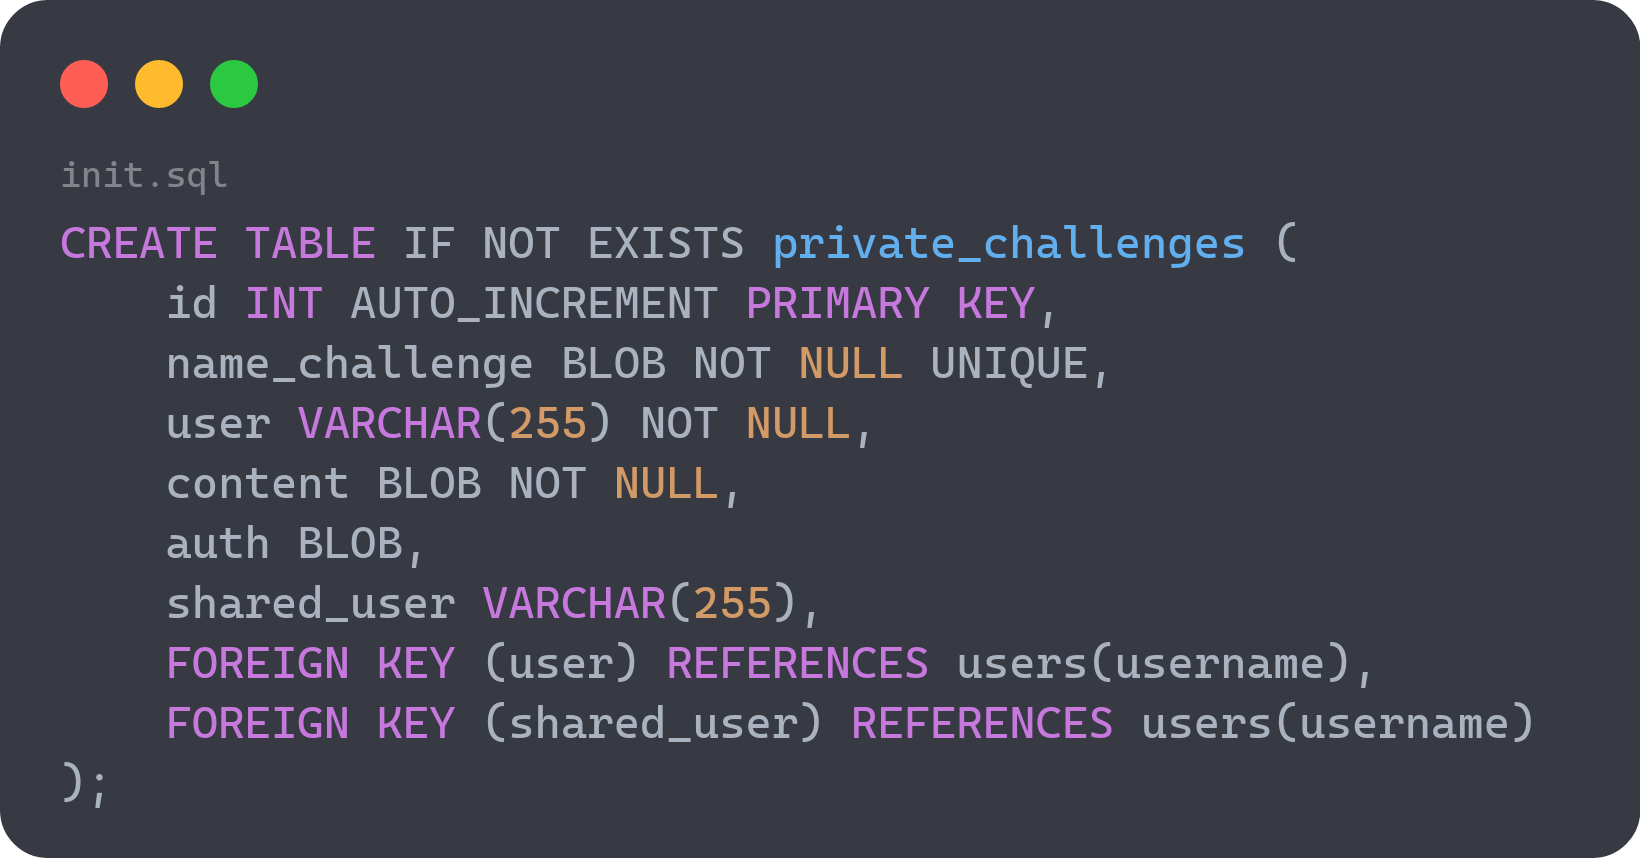
\includegraphics[width=\textwidth]{images/privateChallenge.png}
            \captionof{figure}{Tabla de desafíos privados}
        \end{minipage}
        \hfill
        \begin{minipage}[t]{0.48\textwidth} % Tercio de página
            \centering
            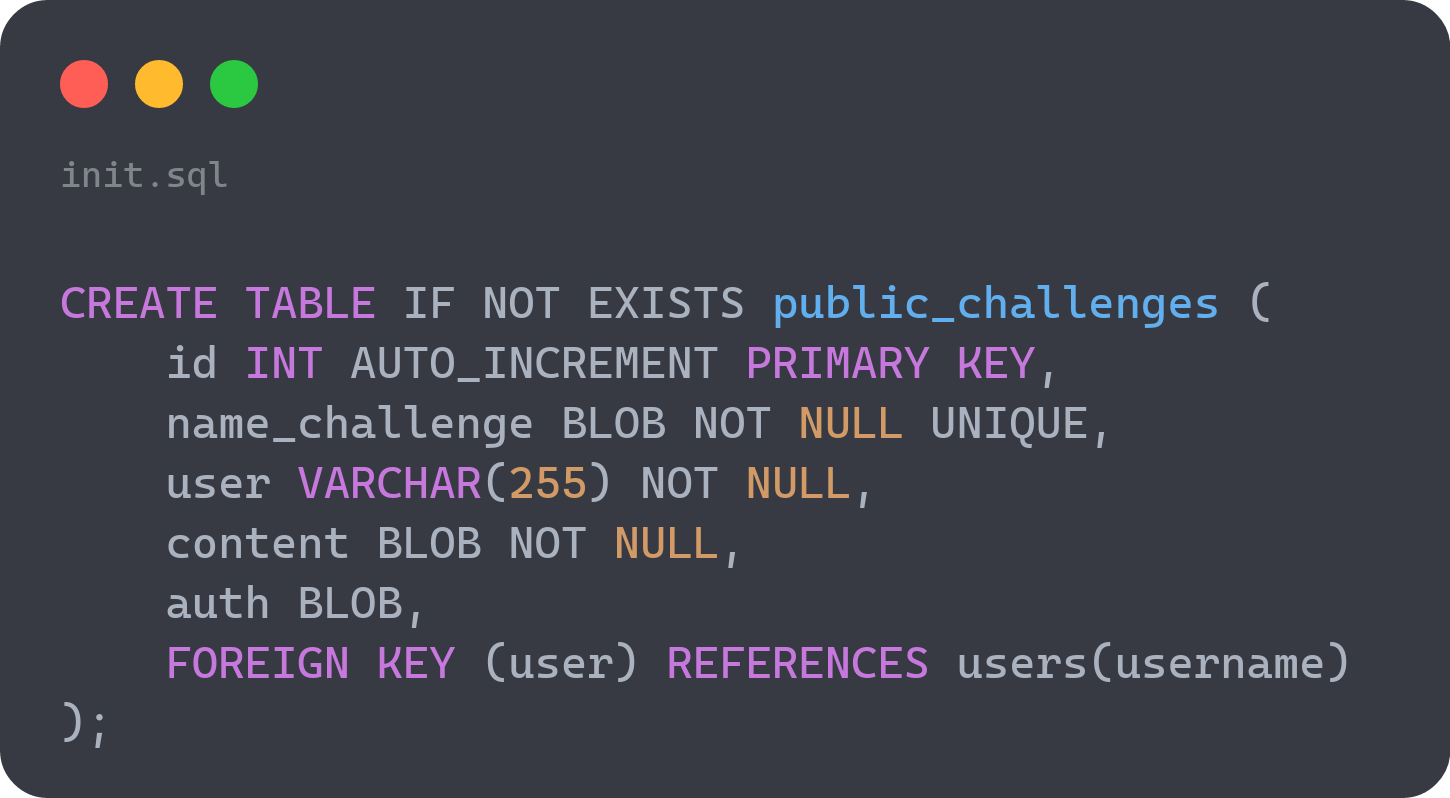
\includegraphics[width=\textwidth]{images/publicChallenge.png}
            \captionof{figure}{Tabla de desafíos públicos}
        \end{minipage}
        \vspace{0.5cm}
        % Segunda fila de imagen (centrada)
        \begin{minipage}[t]{0.7\textwidth} % Tercio de página
            \centering
            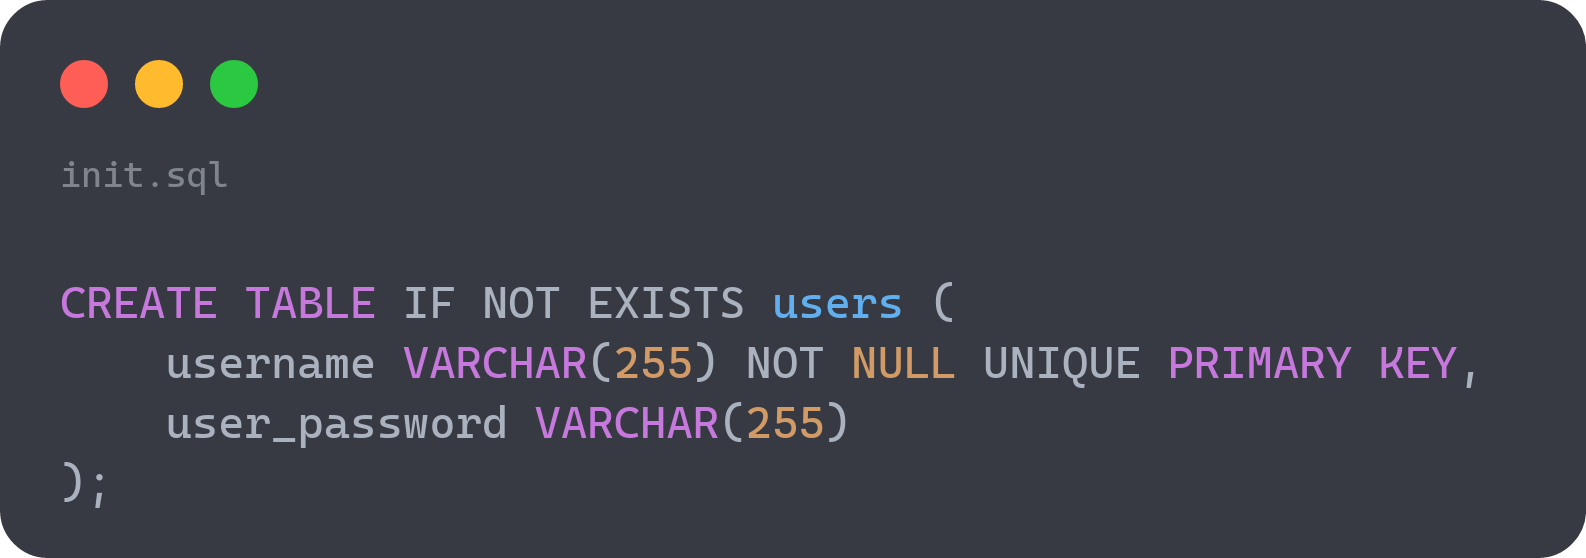
\includegraphics[width=\textwidth]{images/users.png}
            \captionof{figure}{Tabla de usuarios}
        \end{minipage}
    \end{figure}


\subsection{Funciones Hash}
    \label{sec:funcionesHash}
    \centering
    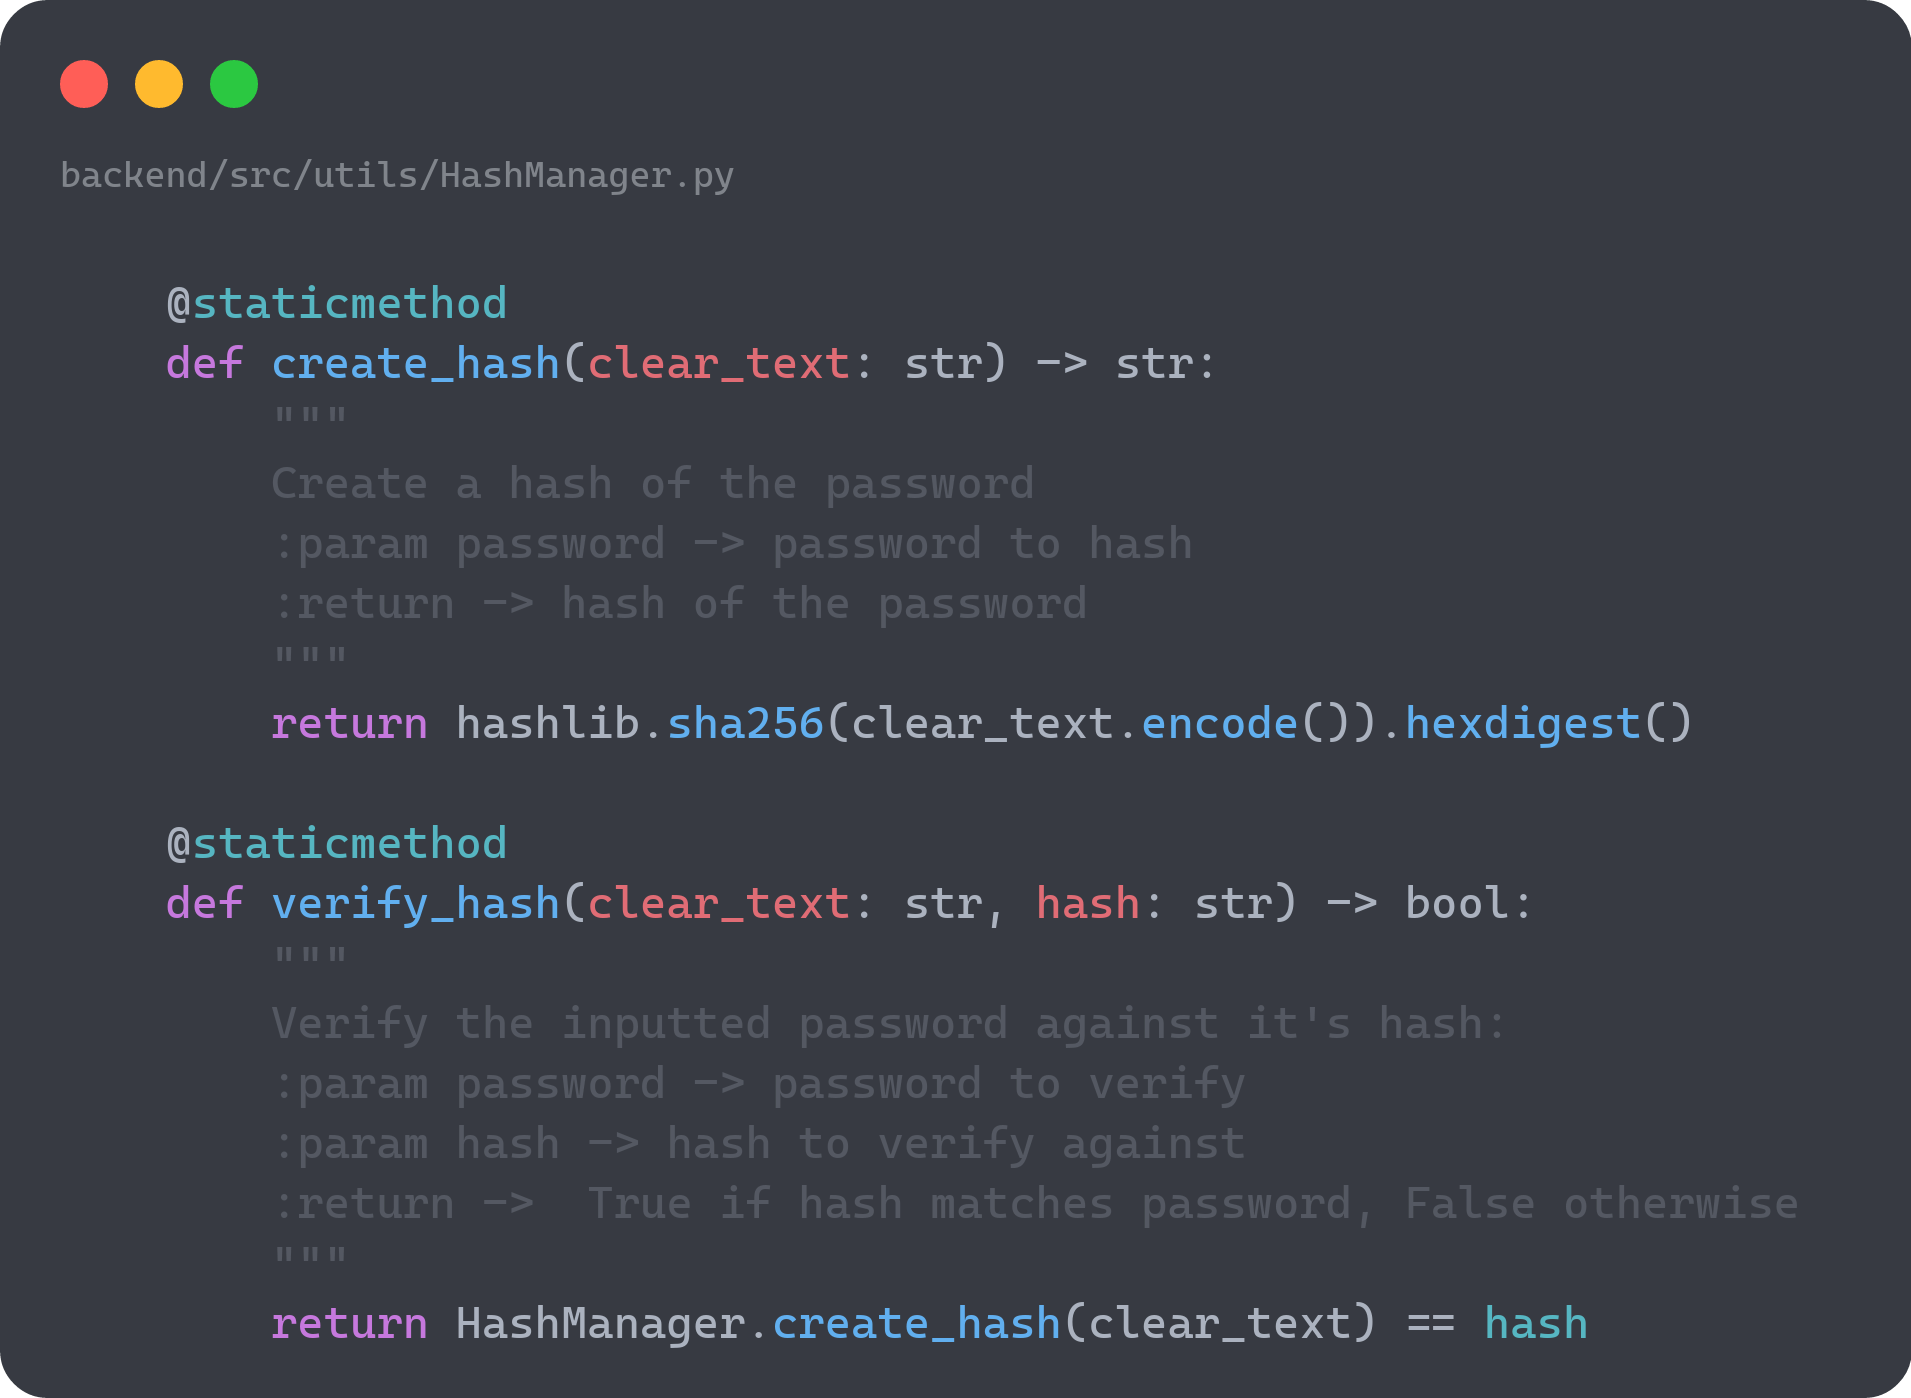
\includegraphics[width=0.8\textwidth]{images/HashFunctions.png} 

\end{document}
